\documentclass[conference]{IEEEtran}
\IEEEoverridecommandlockouts

\usepackage{amsmath,amssymb}
\usepackage{graphicx}
\usepackage{booktabs}
\usepackage{cite}
\usepackage{microtype}
\usepackage{url}
\usepackage{xcolor}
\usepackage[colorlinks=true,linkcolor=blue,citecolor=blue,urlcolor=blue]{hyperref}

\graphicspath{{figures/}}
\renewcommand{\baselinestretch}{0.98}
\setlength{\textfloatsep}{8pt plus 2pt minus 2pt}
\setlength{\floatsep}{6pt plus 2pt minus 2pt}
\setlength{\intextsep}{6pt plus 2pt minus 2pt}
\setlength{\abovecaptionskip}{4pt}
\setlength{\belowcaptionskip}{0pt}

\begin{document}

\title{CREATE: A Closed-Loop Reward Engineering Agent with Training Evidence for Reinforcement Learning}

\author{\IEEEauthorblockN{Anonymous Authors}
\IEEEauthorblockA{Anonymous Submission}}

\maketitle

\begin{abstract}
Evaluating an automatically generated reward normally requires a complete reinforcement-learning training run, but many reward-search pipelines reduce that expensive run to a scalar score. This paper introduces CREATE, a Closed-Loop Reward Editing Agent with Training Evidence, which treats each completed policy-training run as diagnostic evidence for repairing the active reward program. CREATE converts native evaluation outcomes, termination patterns, component activation rates, magnitude shares, and cross-round history into a structured observation; diagnoses one principal reward semantic; applies a bounded L1/L2/L3 edit; and preserves the evidence--action--outcome chain in intervention memory while a best archive guards against later regressions. On LunarLander-v3, CREATE solves all five reward-search lineages within a ten-evaluation budget, whereas budget-matched independent generation and stateless revision solve none. Mechanism ablations show that enriched evidence and hierarchical semantic editing are coupled requirements: removing evidence enrichment reduces success to 2/5, and removing bounded editing reduces success to 0/5. A secondary BipedalWalker-v3 study provides supporting evidence that the same diagnostic loop can transfer to continuous-action locomotion. These results support reward repair as an agentic closed-loop process in which failed training runs become actionable observations rather than discarded outcomes.
\end{abstract}


\begin{IEEEkeywords}
reinforcement learning, reward design, large language models, language agents, training evidence
\end{IEEEkeywords}

\section{Introduction}

Reinforcement learning (RL) depends critically on reward functions that express task intent while providing informative feedback for policy optimization~\cite{sutton2018rl}. Reward shaping can improve credit assignment, but only restricted transformations are guaranteed to preserve the optimal policy~\cite{ng1999policy}. Inverse reward design further shows that a written reward should be treated as imperfect evidence of designer intent rather than as the intent itself~\cite{hadfield2017inverse}. Reward misspecification can therefore produce unsafe or unintended behavior even when the specified signal appears semantically reasonable~\cite{amodei2016concrete}.

Reward engineering is consequently an iterative debugging process rather than a one-shot coding task. Each completed training run produces more than a scalar return: episode length, termination patterns, reward-component activation, magnitude balance, and temporal trends can reveal how the reward program shaped the learned policy. Converting these heterogeneous records into a precise reward modification, however, still requires substantial human analysis.

Code-capable large language models (LLMs) can generate reward programs from task descriptions~\cite{language2rewards,text2reward} and iteratively refine them through training feedback and evolutionary search~\cite{eureka,card,revolve,cotreward}. Diagnostic-driven refinement further treats reward failure as a debugging problem~\cite{wang2026diagnostic}. In parallel, LLMs are increasingly organized as agents that observe, reason, and act across trials, using stored feedback to improve later decisions~\cite{react,reflexion,selfrefine}. These developments motivate an agent-oriented view of reward engineering in which policy training supplies observations and reward-code revision constitutes an external action.

This paper explores an agent-oriented view of reward engineering through CREATE, a \emph{Closed-Loop Reward Engineering Agent with Training Evidence}. CREATE places a reward-engineering agent above an inner RL policy learner. After each policy-training run, the reward-engineering agent uses explicit tool calls to inspect training feedback, reward and lineage history, and component-level trends while it reasons about the next repair. It then diagnoses one principal semantic failure and applies a localized edit: L1 tunes parameters, L2 refactors one semantic, and L3 redesigns the reward structure after repeated local failure. Intervention memory retains this evidence chain across rounds, while a separate best archive protects the strongest solution from later exploratory regressions.

Experiments on LunarLander-v3 compare CREATE against budget-matched independent generation and baseline, with two mechanism ablations isolating evidence enrichment and hierarchical semantic editing. BipedalWalker-v3 provides a secondary cross-task validation. Under a ten-evaluation budget, the experiments demonstrate that structured observation, persistent state, and bounded reward actions convert failed policy training into reliable reward repair.

\section{Related Work}
\subsection{Reward Engineering for Reinforcement Learning}
Reward shaping augments task objectives with intermediate signals that improve credit assignment while preserving the optimal policy only under restricted transformations~\cite{ng1999policy}. Inverse reward design treats a specified reward as imperfect evidence of designer intent and highlights the gap between written objectives and desired behavior~\cite{hadfield2017inverse}. More broadly, reward misspecification can produce unsafe or unintended behavior even when the reward appears semantically reasonable~\cite{amodei2016concrete}. These results motivate methods that treat reward engineering as an iterative debugging problem rather than a one-shot specification step.

\subsection{LLM-Based Reward Generation and Refinement}
LLMs can map task descriptions to executable reward code. Language to Rewards demonstrates language-conditioned reward generation for robotic skill synthesis~\cite{language2rewards}. Text2Reward frames reward shaping as interpretable program synthesis from language instructions~\cite{text2reward}. Eureka combines reward-code generation with evolutionary optimization and component-level feedback~\cite{eureka}. CARD incorporates dynamic feedback into LLM-driven reward design~\cite{card}. REvolve studies reward evolution with human feedback in the loop~\cite{revolve}. A chain-of-thought reward-engineering approach shows that explicit reasoning traces can improve reward-design transparency~\cite{cotreward}. Diagnostic-driven refinement treats reward failure as a debugging problem and uses training diagnostics for targeted revision~\cite{wang2026diagnostic}. Collectively, these methods show that training feedback supports reward revision beyond one-shot generation.

\subsection{LLM Agents and Agentic Reward Engineering}
Language-agent research organizes LLMs to maintain state and act in external processes. ReAct couples reasoning with tool-mediated actions~\cite{react}. Reflexion stores verbal feedback as episodic experience for later decisions~\cite{reflexion}. Self-Refine shows how iterative self-feedback can improve generated outputs without parameter updates~\cite{selfrefine}. These mechanisms are entering reward design: RF-Agent formulates reward construction as sequential decision making~\cite{rfagent}, and STRIDE applies agentic reward engineering to humanoid locomotion~\cite{stride}. CREATE follows this direction but centers agency on instrumented policy training: the reward-engineering agent calls tools over training records, reasons over the returned evidence, and commits to a semantically localized action measured by the next complete training run.

\section{CREATE}
\label{sec:method}
CREATE comprises an outer reward-editing agent and an underlying RL agent. The RL agent interacts with the environment and learns a policy under the current generated reward, whereas CREATE treats each completed policy-training and native-evaluation run as one reward-design round. As shown in Fig.~\ref{fig:create_framework}, tool-assisted evidence processing organizes the resulting records before the reward-editing agent diagnoses the current reward and executes a validated edit.

\begin{figure*}[!t]
\centering
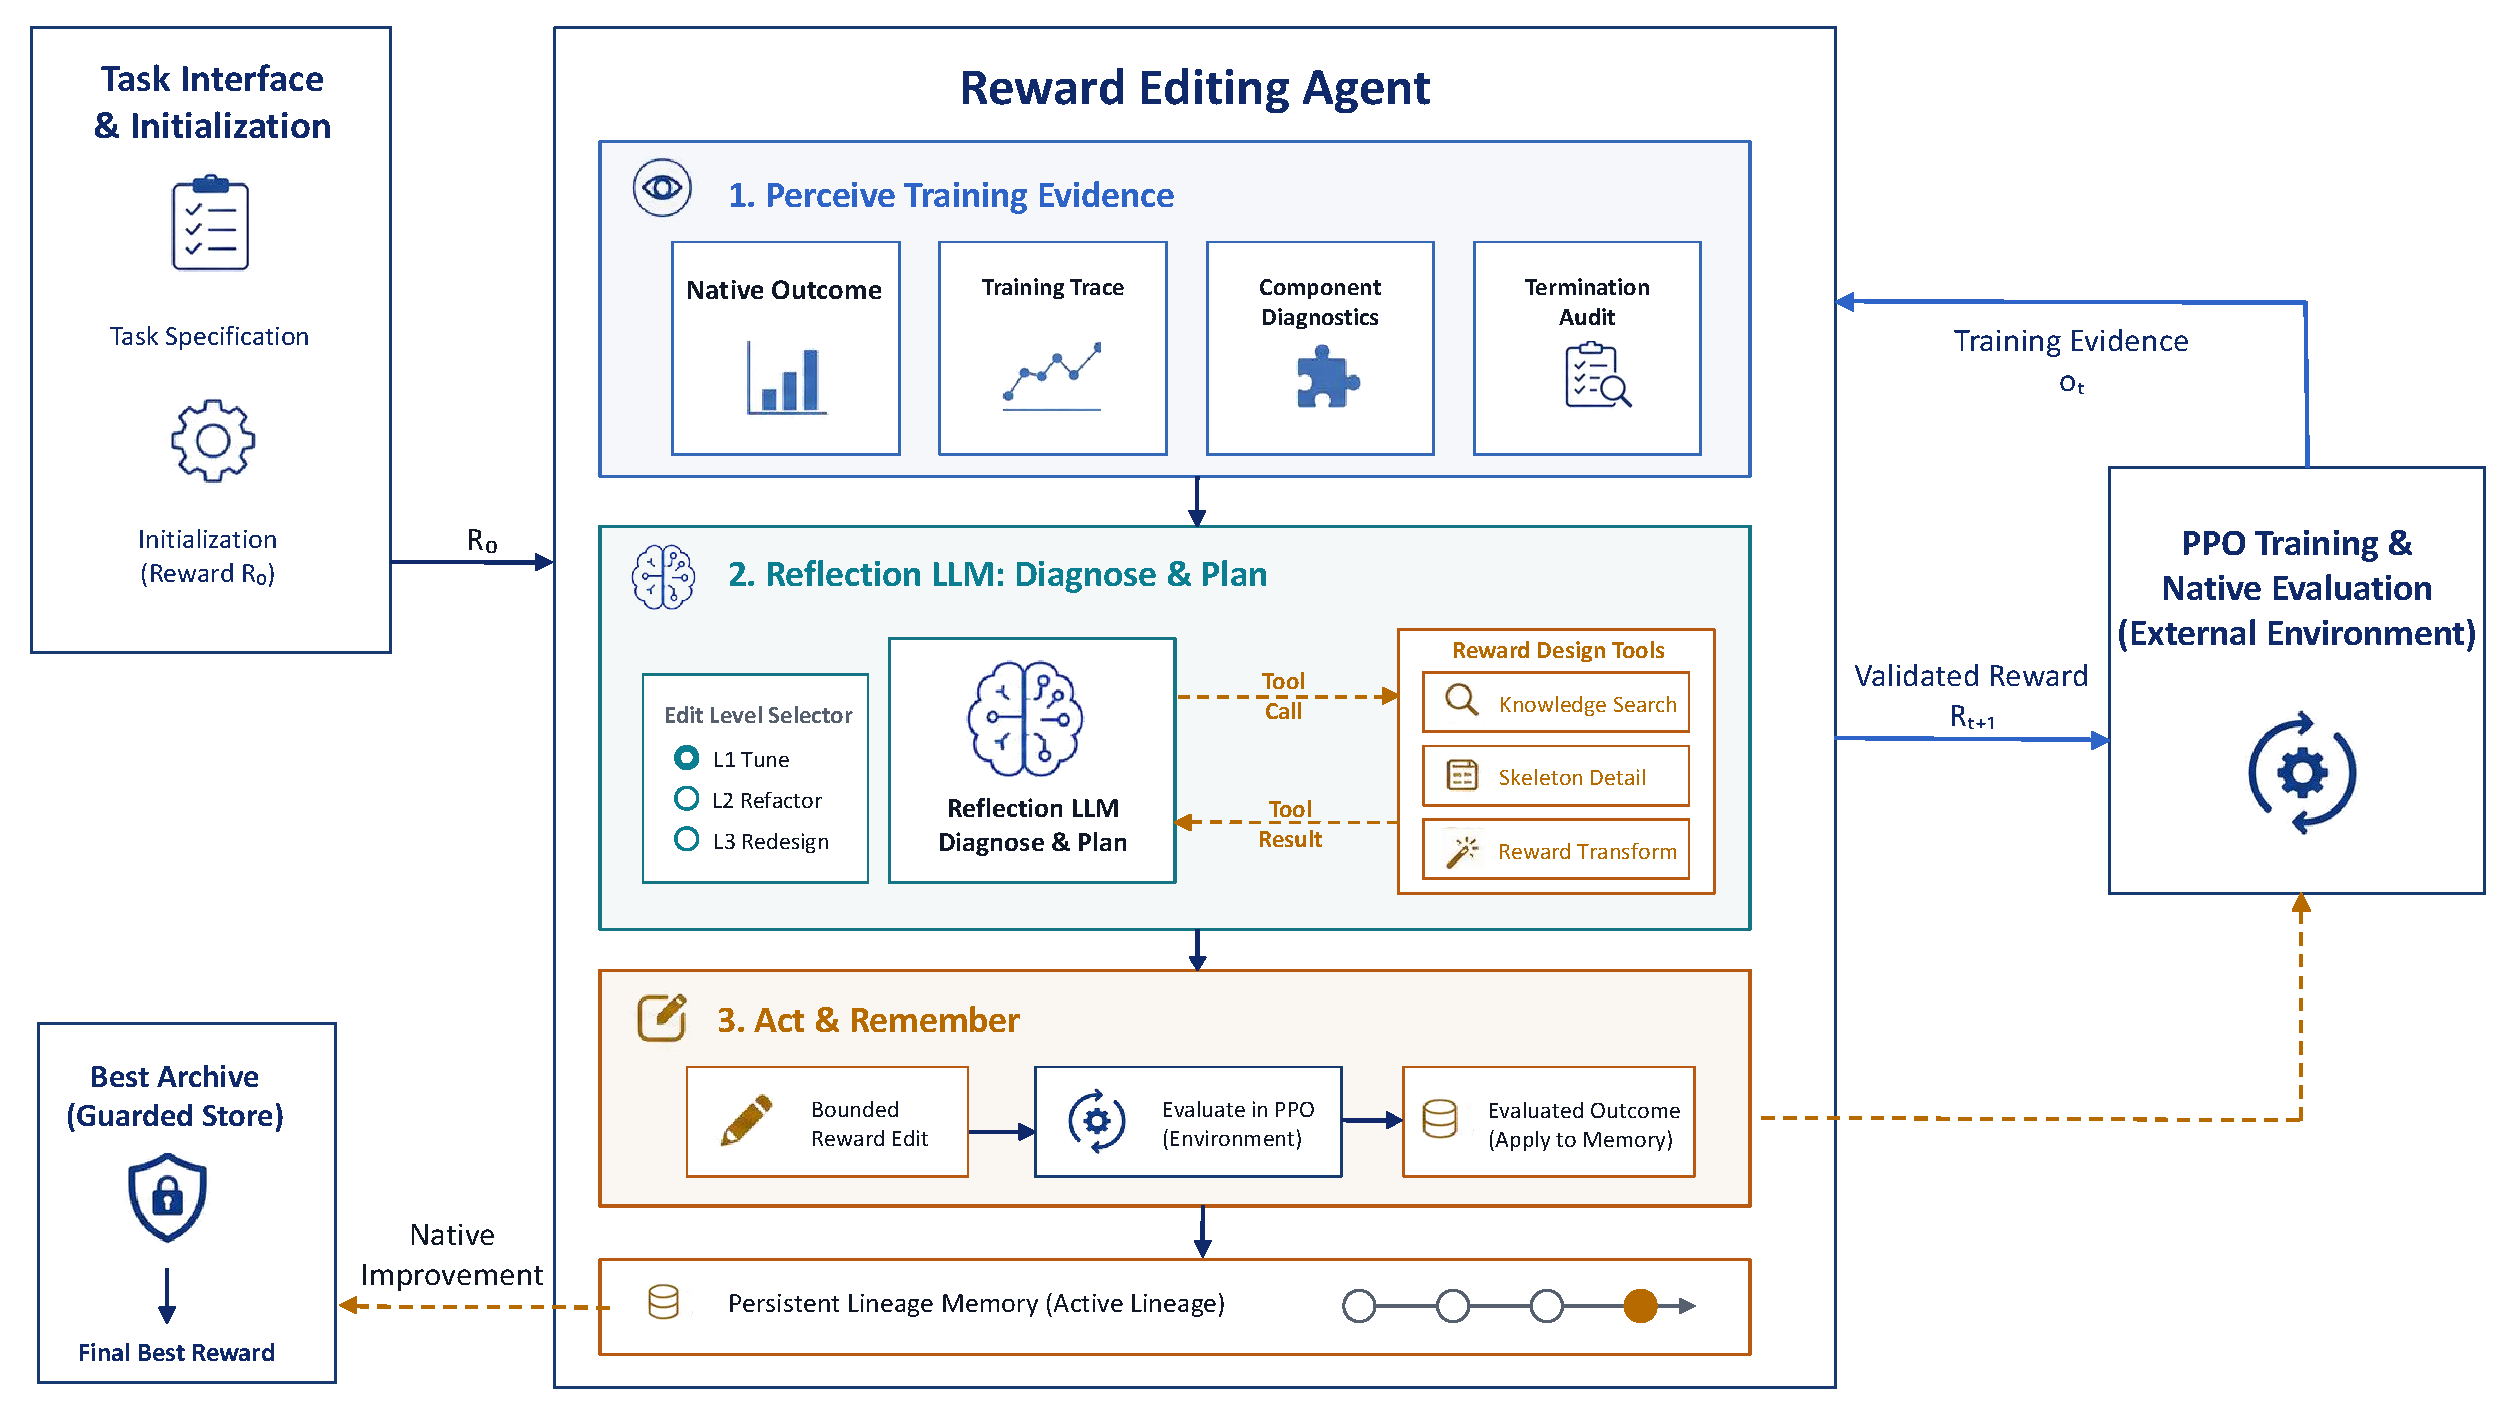
\includegraphics[width=0.98\textwidth]{cretae_framework.pdf}
\caption{Overview of CREATE. The underlying RL agent learns under the current generated reward. Tool-assisted evidence processing retrieves and compresses relevant training and lineage records, while the reward-editing agent remains responsible for failure diagnosis, semantic localization, intervention-level selection, and reward modification. Persistent memory records intervention outcomes, and the best archive retains the reward program with the highest native-task performance.}
\label{fig:create_framework}
\end{figure*}

The resulting observe--reflect--act loop is written as
\begin{equation}
\begin{aligned}
O_t&=\Phi_{\mathcal T}(\mathcal D_t),\\
(H_t,A_t)&=\Psi(R_t,O_t,M_t,B_t),\\
R_{t+1}&=\mathcal U(R_t,A_t),
\end{aligned}
\label{eq:agent_loop}
\end{equation}
where the training record $\mathcal D_t$ is retrieved and compressed into observation $O_t$ through evidence tools. This processing stage organizes information but does not select a reward edit. The reward-editing agent combines $O_t$ with the current reward $R_t$, intervention memory $M_t$, and best archive $B_t$ to produce reflection $H_t$, reward action $A_t$, and the next executable reward program $R_{t+1}$.

\subsection{Task Understanding and Reward Initialization}
\label{sec:init}
Given the task description, environment interface, and reward-code constraints, CREATE identifies the principal behavior semantics and instantiates them as named reward components. The initial reward is
\begin{equation}
R_0(s,a,s')=\sum_{i=1}^{m_0}w_i^{(0)}r_i^{(0)}(s,a,s'),
\label{eq:initial_reward}
\end{equation}
where each component represents a behavior semantic such as task progress, stability, target events, or action cost. Named components are logged independently during training, enabling component-level diagnosis in later rounds. Generated code is checked for interface and execution validity before policy training; prompts and validation rules are provided in the supplementary material.

\subsection{Training-Evidence-Driven Observe--Reflect--Act}
At iteration $t$, the underlying RL agent optimizes the generated reward, while CREATE evaluates the learned policy with the environment-native objective:
\begin{equation}
\begin{aligned}
\pi_t &= \arg\max_{\pi}\;\mathbb E_{\tau\sim\pi}
\left[\sum_{k=0}^{H-1}\gamma^kR_t(s_k,a_k,s_{k+1})\right],\\
J_t &= \frac{1}{N}\sum_{n=1}^{N}\sum_{k=0}^{H_n-1}
 r_{\mathrm{env}}(s_k^{(n)},a_k^{(n)},s_{k+1}^{(n)}).
\end{aligned}
\label{eq:train_eval}
\end{equation}
Thus, the generated reward shapes policy learning, whereas the native objective measures task completion. Each run produces episode outcomes, termination patterns, component activation and scale, temporal dynamics, and differences from the preceding reward version. An auxiliary tool-using subagent retrieves and compresses these records into a structured evidence summary. It reports what occurred during training but does not recommend coefficient changes, select an intervention level, or modify reward code.

Component statistics serve as diagnostic cues rather than fixed editing rules. Persistent inactivity may indicate an unreachable gate or sparse formulation; excessive activation and magnitude may reveal a dominant proxy; frequent activation with weak contribution may indicate insufficient scale, saturation, or an ineffective mathematical form. The reward-editing agent combines these cues with policy outcomes, reward source code, and prior interventions to identify one principal reward semantic for the next edit:
\begin{equation}
A_t=(q_t,\ell_t,\Delta_t),
\qquad
\operatorname{supp}(\Delta_t)\subseteq\mathcal C(q_t),
\label{eq:semantic_action}
\end{equation}
where $q_t$ denotes the selected semantic, $\ell_t$ the edit level, and $\mathcal C(q_t)$ the components and parameters implementing that semantic. An ordinary action may add or remove a component, adjust its weight or gate, or replace its mathematical form. Related components may be adjusted jointly when they express the same semantic, but independent design intents are not mixed within one ordinary revision. L1 calibrates coefficients, thresholds, or gates; L2 adds, removes, or refactors components while preserving the target semantic; and L3 replans the reward structure after repeated local failure.

\subsection{Intervention Memory and Best-Reward Selection}
After each round, CREATE records the observation, diagnosed semantic, reward action, expected change, and subsequent outcome in persistent intervention memory. This history supports comparison across rounds and discourages repeated unsuccessful edits. The best archive is maintained separately from the active lineage to prevent later regressions from overwriting a previously discovered solution. After at most $K$ reward evaluations, CREATE returns
\begin{equation}
t^*=\arg\max_{0\leq t<K}J_t,
\qquad R^*=R_{t^*}.
\label{eq:best_reward}
\end{equation}
The selected reward--policy pair is subsequently evaluated on independent episode seeds to assess stability.

\subsection{Summary}
\label{sec:method_summary}

Together, the three-stage architecture---evidence processing (Eq.~\ref{eq:agent_loop}), semantic diagnosis and bounded editing (Eq.~\ref{eq:semantic_action}), and intervention memory with best-reward selection (Eq.~\ref{eq:best_reward})---forms a closed diagnostic loop. Each completed policy-training run produces component-level evidence that reveals \emph{which} semantic failed and \emph{how}; the editor commits to a targeted intervention on that semantic alone; and the next training run measures whether the diagnosis was correct. Intervention memory preserves this chain across rounds, while the best archive guards against regression. The experiments in Section~\ref{sec:exp_procedure} and~\ref{sec:results} test whether this diagnostic architecture can convert failed policy training into reliable reward repair under a fixed evaluation budget.

\section{Experimental Procedure}
\label{sec:exp_procedure}

This section details the experimental protocol that implements the CREATE framework described in Section~\ref{sec:method}. We describe the setup, the six conditions under comparison, and the training and evaluation pipeline. Results are deferred to Section~\ref{sec:results}.

\subsection{Experimental Setup and Configuration}
\label{sec:exp_setup}

Experiments are conducted on two Gymnasium environments. LunarLander-v3 serves as the primary benchmark for baseline comparison and mechanism ablation; BipedalWalker-v3 provides a secondary validation on continuous-action locomotion. Every reward program trains a freshly initialized PPO policy through Stable-Baselines3. LunarLander uses $10^6$ environment steps per candidate and BipedalWalker uses $5\times10^6$, with four vectorized environments inside each policy-training job. The computational infrastructure comprises two NVIDIA GeForce RTX 3090 GPUs (24\,GB each), with DeepSeek V4 Pro serving as the LLM backbone for all LunarLander conditions. Full prompts, model settings, hyperparameters, and per-seed traces are provided in the supplementary material.

\subsection{Condition Definitions}
\label{sec:conditions}

Six conditions are compared on LunarLander-v3 under a shared LLM backbone, environment description, reward interface, code checks, and PPO budget. Each condition contains five independent reward-search lineages and at most ten complete reward evaluations, so that every condition operates under the same total policy-training cost.

\textbf{Single-shot generation} evaluates only the initial reward produced by CREATE's task-understanding phase (Section~\ref{sec:init}), without subsequent observation or revision.

\textbf{Independent-10} generates ten unrelated initial reward candidates, each from an independent invocation of the reward-initialization phase, and evaluates each with a separate policy-training run. The best candidate is selected post hoc. This condition spends the same maximum number of evaluations as CREATE but without cross-round information flow.

\textbf{Stateless iterative revision} repeatedly revises the current reward from basic current-round feedback (native fitness, episode length, termination statistics, component episode sums), but removes the evidence organizer, intervention memory, cross-round component comparison, and hierarchical semantic editing.

\textbf{CREATE w/o evidence enrichment} retains the full loop, memory, best archive, and hierarchical editing, but removes the tool-using evidence organizer: the editor receives native fitness, episode length, termination statistics, and component episode sums, but lacks activation rates, magnitude shares, temporal trends, and cross-round summaries.

\textbf{CREATE w/o hierarchical editing} retains enriched evidence, memory, and the best archive, but removes the semantic-localization constraint (Eq.~\ref{eq:semantic_action}), allowing unconstrained multi-component rewrites.

\textbf{CREATE} runs the complete architecture described in Section~\ref{sec:method}.

\subsection{Training and Evaluation Protocol}
\label{sec:training_protocol}

Each reward-design round consists of a complete PPO training run followed by native evaluation. The policy is optimized with the generated reward $R_t$, whereas candidate quality is measured only by the untouched environment reward $r_{\mathrm{env}}$ (Eq.~\ref{eq:train_eval}). We define \emph{search fitness} as the mean undiscounted native episodic return over 20 fixed evaluation episodes and \emph{best search fitness} as the largest value retained within a lineage. After reward selection, the returned policy is evaluated over 100 unseen episodes; this is reported as \emph{test fitness}. The task-solving thresholds are 200 for LunarLander and 300 for BipedalWalker.

Between rounds, the evidence organizer (Eq.~\ref{eq:agent_loop}, $\Phi_{\mathcal T}$) compresses training records into a structured summary. The reward-editing agent then selects one principal semantic, chooses an edit level (L1/L2/L3), and applies a bounded modification (Eq.~\ref{eq:semantic_action}). The modified program is validated before the next round. The best archive is updated only when a new candidate exceeds the current incumbent in native search fitness (Eq.~\ref{eq:best_reward}). On BipedalWalker-v3, only the complete CREATE workflow is evaluated; no baseline or ablation comparison is conducted on that task.

\section{Results and Analysis}
\label{sec:results}

\subsection{Reward Search Under a Matched Training Budget}
\label{sec:reward_search}

\begin{table}[t]
\caption{Seed-level LunarLander best-search fitness.}
\label{tab:lander_main}
\centering
\scriptsize
\setlength{\tabcolsep}{2.5pt}
\begin{tabular}{@{}lrrrrrr@{}}
\toprule
Condition & s0 & s1 & s2 & s3 & s4 & Mean \\
\midrule
\multicolumn{7}{@{}l}{\emph{Budget-matched baselines}}\\
Independent-10 & -13.1 & 170.8 & 55.1 & -106.7 & -109.7 & $-0.7\pm118.1$ \\
Baseline & 25.4 & -5.0 & -10.1 & 151.3 & 58.9 & $44.1\pm66.0$ \\
CREATE & \textbf{224.2} & \textbf{240.6} & \textbf{220.2} & \textbf{253.7} & \textbf{206.1} & $\mathbf{229.0\pm18.5}$ \\
\midrule
\multicolumn{7}{@{}l}{\emph{Mechanism ablations}}\\
w/o evidence & \textbf{239.5} & 170.4 & -110.1 & 115.5 & \textbf{259.5} & $135.0\pm148.4$ \\
w/o hierarchy & 169.9 & 130.6 & 71.1 & 59.2 & 140.3 & $114.2\pm47.3$ \\
CREATE & \textbf{224.2} & \textbf{240.6} & \textbf{220.2} & \textbf{253.7} & \textbf{206.1} & $\mathbf{229.0\pm18.5}$ \\
\bottomrule
\end{tabular}
\end{table}

\textbf{Search breadth alone does not produce reliable reward repair.} Table~\ref{tab:lander_main} reports per-seed best search fitness under a ten-evaluation budget, with bold entries crossing the 200 threshold. Independent-10 evaluates ten unrelated candidates without cross-round information flow, yet solves no lineage---ruling out that candidate count alone drives improvement. The iterative conditions share the same task facts, environment interface, reward-generation protocol, and PPO budget; subsequent differences therefore reflect each architecture's capacity to convert training outcomes into better reward functions.

\textbf{Iterative rewriting without tool-use evidence or memory produces non-monotonic progress.} Baseline retains sequential LLM invocation but removes tool access, memory, and editing constraints. It solves no lineage, and in three seeds the initial reward outperforms every subsequent revision. Without component-level diagnostics or memory, the LLM cannot distinguish a poorly calibrated coefficient from a fundamentally wrong semantic---each rewrite is effectively a guess. CREATE, by contrast, solves every lineage, demonstrating that agentic evidence seeking, not repeated invocation, drives reliable repair.

\begin{figure}[!htbp]
\centering
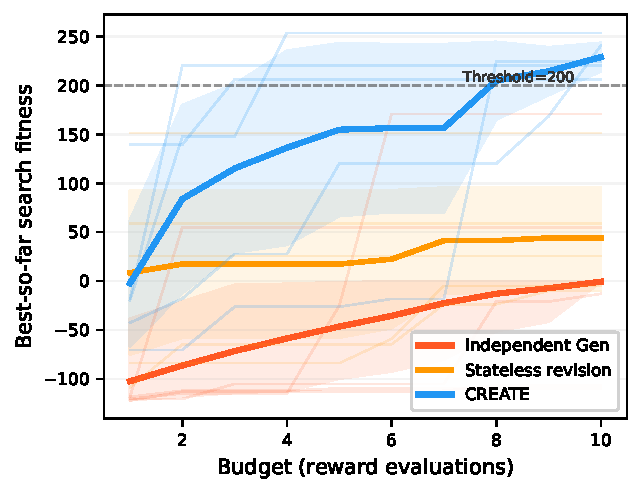
\includegraphics[width=0.98\columnwidth]{fig2_budget_curve.pdf}
\caption{Best-so-far LunarLander search fitness under a matched policy-training budget. Each curve averages five lineages after retaining the incumbent within each lineage; the dashed line denotes the task-solving threshold.}
\label{fig:budget_curve}
\end{figure}

Fig.~\ref{fig:budget_curve} reveals the qualitative gap: Independent-10 improves by chance, Baseline plateaus, and CREATE progressively raises its incumbent. The distinction is whether each training run becomes diagnostic evidence rather than a binary outcome. Fig.~\ref{fig:heldout_ablation}(a) shows that the same gap appears at the per-lineage level.

\subsection{Mechanism Ablations}
\label{sec:mechanism_ablations}

We now isolate \emph{why} the closed loop works by testing two mechanism hypotheses from Section~\ref{sec:method}.

\textbf{Tool use enables agentic diagnosis.} Activation rates, magnitude shares, and temporal trends let the reward-engineering agent distinguish mechanistically distinct failure modes---for instance, an inactive component could be unreachable, too weak, or behaviorally irrelevant, and a scalar sum cannot tell them apart.

Without tool-use access, the reward-engineering agent can consult only scalar current-round feedback. Table~\ref{tab:lander_main} shows that this variant solves only two of five lineages, with high dispersion and one lineage that remains negative throughout. Aggregate scores can support occasional repair but cannot distinguish \emph{why} a component failed: \emph{what} evidence the agent can inspect determines \emph{which} diagnoses it can form.

\textbf{Bounded reward actions enable single-trial attribution.} Eq.~\ref{eq:semantic_action} formalizes the semantic-localization constraint that makes each retraining run a controlled test of one intervention. This matters because reward revision is not ordinary program repair: an LLM can analyze code and diagnostics, but the policy consequence of changing reward weights, gates, or mathematical forms appears only after black-box RL training~\cite{wang2026diagnostic}.

Without bounded actions, the agent retains tool-returned evidence and memory but may issue unconstrained multi-component rewrites. Table~\ref{tab:lander_main} shows that this variant solves no lineage, while Fig.~\ref{fig:heldout_ablation}(b) shows the same failure pattern visually. If several components are retuned or refactored together, a failed next run gives no stable diagnostic target: the agent may react by changing other components, coupling unrelated hypotheses and severing the evidence--action--outcome chain. The ablation therefore degenerates into metrics-conditioned trial and error, not experience-guided diagnosis; each $10^6$-step run must stay tied to one falsifiable reward hypothesis.

\begin{figure}[!htbp]
\centering
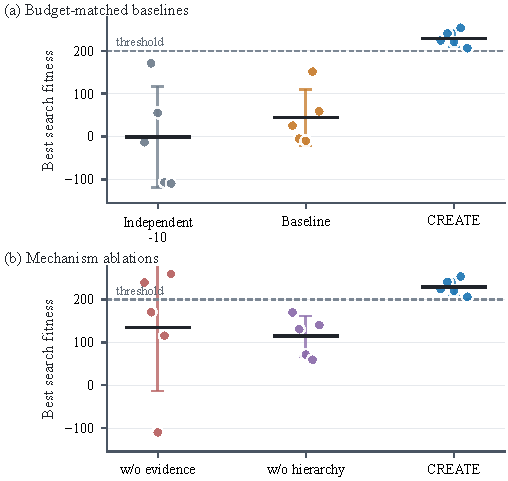
\includegraphics[width=0.98\columnwidth]{fig_heldout_ablation_combined.pdf}
\caption{LunarLander per-lineage search outcomes. (a) Independent-10, Baseline, and CREATE under a matched budget. (b) CREATE compared with the two mechanism ablations. Dots are lineages, black bars are means, whiskers denote standard deviations, and the dashed line denotes the task threshold.}
\label{fig:heldout_ablation}
\end{figure}

Fig.~\ref{fig:heldout_ablation}(b) shows that tool-mediated evidence and bounded actions are coupled requirements. Evidence-poor repair is initialization-dependent, and unconstrained rewriting remains below threshold in every lineage. Full CREATE combines 5/5 solutions with a tight distribution, aligning high success rate with reliable attribution.

\subsection{Agentic Diagnosis from Tool-Returned Evidence}
\label{sec:evidence_to_edit}

We examine \emph{how} the reward-engineering agent turns tool-returned evidence into a diagnosis and intervention through the most representative seed-0 trajectory in Fig.~\ref{fig:repair_patterns}. This lineage contains both collapse and recovery; complete traces and additional component-evidence heatmaps are provided in the appendix.

\begin{figure}[!htbp]
\centering
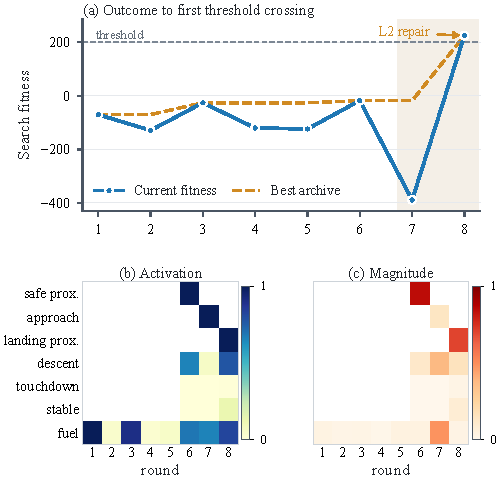
\includegraphics[width=0.98\columnwidth]{fig4_traces.pdf}
\caption{Auditable CREATE repair for LunarLander seed~0. (a) Current fitness and the protected best archive. (b) Component activation rates across rounds. (c) Component magnitude shares used during diagnosis.}
\label{fig:repair_patterns}
\end{figure}

\textbf{Diagnostic trajectory.} Subfigures b and c separate three kinds of components: guidance signals such as safe, approach, and landing proximity; safety or cost terms such as descent and fuel; and landing-quality events such as touchdown and stable. Iterations 1--5 fail to produce stable landing, with the best score still below zero. Before iteration~6, the agent observes from the training records that distance progress is active while episodes terminate early; the queried reward-design tools map this pattern to proxy misalignment and missing safe-descent feedback. The selected L2 action removes raw distance reduction and introduces state-based safe proximity, descent safety, touchdown, and stable-landing components, visible as new rows in subfigure b. Iteration~6 improves to $-18.3$ and survives much longer, giving memory a useful but still unsolved reference point.

\textbf{Collapse and recovery.} The next reward version changes the approach signal back to a delta-style shaping term and collapses at iteration~7 to $-388.7$. The tools then expose the failure signature reflected in subfigures b and c: touchdown and stable-landing components are not activated, approach shaping contributes negatively, and descent safety appears only rarely but with large penalty share. Rather than discarding the entire reward, the agent compares against iteration~6 and selects an L2 repair: replace the unstable delta signal with a bounded landing-proximity term that combines horizontal centering with a height factor, while keeping safety and landing components. Iteration~8 reaches 224.2, and subfigure a shows the best archive preserving this recovered solution through later exploratory regression.

\textbf{Mechanism summary.} The case illustrates the full CREATE loop: tool calls inspect lineage state, including reward code, prior diagnoses, component activation, magnitude balance, and previous outcome; memory makes iteration~6 the recovery anchor and iteration~7 negative evidence; and the agent returns to the best preserved reward family. It then changes only the unstable semantic, so recovery is diagnostic rather than a fresh regeneration attempt.

\subsection{Cross-Task Validation}
\label{sec:cross_task}

BipedalWalker-v3 validates CREATE on continuous-action locomotion as a secondary domain with a different action space and gait-control reward structure. The ten-evaluation cap and input protocol remain unchanged, but the reward semantics shift from landing to forward gait and stability. Table~\ref{tab:bipedal} reports the first reward version that crosses the task threshold, where $v$ denotes the evaluated version.

\begin{table}[!h]
\caption{BipedalWalker-v3 CREATE search results.}
\label{tab:bipedal}
\centering
\footnotesize
\setlength{\tabcolsep}{4.0pt}
\begin{tabular}{@{}lccc@{}}
\toprule
Seed & Initial fitness & First $v\!\geq\!300$ & Best search \\
\midrule
0 & 270.7 & $v_2$ & 320.0 \\
1 & 280.5 & $v_2$ & 313.7 \\
2 & 272.1 & $v_2$ & 307.9 \\
3 & 290.0 & $v_2$ & 311.1 \\
4 & 103.0 & $v_3$ & 304.9 \\
\midrule
Mean & $243.26\pm70.45$ & 2.2 versions & $311.54\pm5.17$ \\
\bottomrule
\end{tabular}
\end{table}

All five BipedalWalker lineages cross the threshold within three evaluated reward versions, and the selected policies obtain $310.82\pm5.03$ test fitness over unseen episodes. Four lineages begin near the threshold and mainly require calibration; seed~4 starts from 103.0 and reaches 304.9 after one additional repair round. This secondary result summarizes the cross-task evidence: the same observe--remember--act workflow remains operational when reward repair shifts from discrete landing semantics to continuous gait control.

\section{Conclusion}
This study presented CREATE, a closed-loop reward engineering agent that turns completed policy-training runs into diagnostic observations. On LunarLander-v3, CREATE solved all five lineages under a ten-evaluation budget, while budget-matched independent generation and baseline solved none. Ablations show that tool-use observation and bounded reward actions must work together, and BipedalWalker-v3 indicates that the observe--remember--act loop can extend beyond discrete landing. These results position diagnostic reward repair as a practical path for agentic reward engineering. Future work can make the loop more perceptive and efficient: monitor training convergence to terminate unpromising reward programs early, add visual rollout evidence so the agent can inspect behavioral failure modes, and connect the same repair loop to stronger policy optimizers and harder robotic tasks.


\bibliographystyle{IEEEtran}
\bibliography{references,references_extra}
\end{document}
